%every chapter wil be split into a new document. For the sake of the structure, this one_doc strategy is held up
\chapter{Application Area and Goals}
\label{cha:area_goals}
\section{Introduction}
\begin{itemize}
	\item Problem Statement and idea behind the project
	\item General introduction similar to Project outline
\end{itemize}

\section{Theoretical framework}
\begin{itemize}
	\item keep it small
	\item roughly 1 Page
\end{itemize}
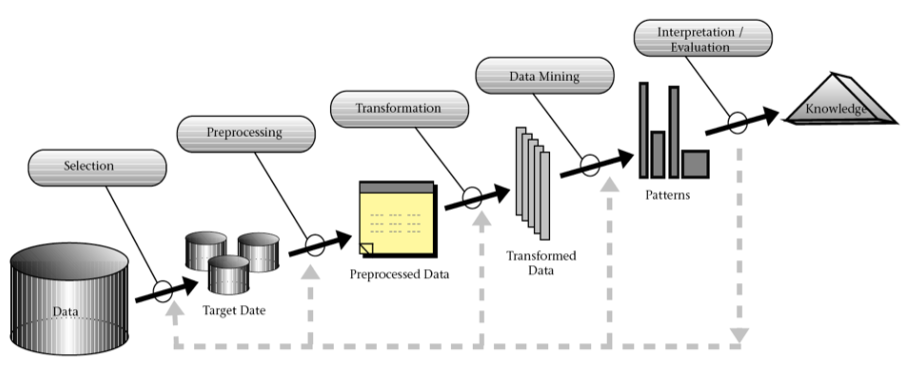
\includegraphics[width=\textwidth]{images/DM_Process.png}



\chapter{Data Selection}
\label{cha:data_selection}
\begin{itemize}
	\item In slides named: "structure and size of data"
	\item min. 1 Page
	\item Selection: 
	\begin{itemize}
		\item What data is available?
		\item What do I know about the provenance of the data?
		\item What do I know about the quality of the data?
	\end{itemize}
	\item Exploration
	\begin{itemize}
		\item Get an intitial understanding of the data
		\item Calculate basic summarization statistics
		\item Visualize the data
		\item Identify data problems such as outliers, missing values, duplicate records
	\end{itemize}
\end{itemize}



\chapter{Preprocessing and Transformation}
\label{cha:preprocessing_transformation}
\begin{itemize}
	\item Transform data into a representation that is suitable for the chosen data mining methods
	\begin{itemize}
		\item number of dimensions
		\item scales of attributes (nominal, ordinal, numeric)
		\item amount of data (determines hardware requirements)
	\end{itemize}
	\item Methods
	\begin{itemize}
		\item Aggregation, sampling
		\item Dimensionality reduction / feature subset selection
		\item Attribute transformation / text to term vector
		\item Discretization and binarization
	\end{itemize}
	\item Good data preparation is key to producing valid and reliable models
	\item Data preparation estimated to take 70-80\% of the time and effort of a data mining project!
\end{itemize}



\chapter{Data Mining}
\label{cha:data_mining}
\begin{itemize}
	\item Input: Preprocessed Data
	\item Output: Model / Patterns
\end{itemize}

\begin{enumerate}
	\item Apply data mining method
	\item Evaluate resulting model / patterns (using P, R, F1, not accuracy)
	\item Iterate:
	\begin{itemize}
		\item Experiment with different parameter settings
		\item Experiment with different alternative methods – Improve preprocessing and feature generation – Combine different methods
	\end{itemize}
\end{enumerate}

\section{Algorithms}



\chapter{Interpretation / Evaluation}
\label{cha:interpretation_evaluation}
\begin{itemize}
	\item Output of Data Mining
	\begin{itemize}
		\item Patterns
		\item Models
	\end{itemize}
	\item In the end, we want to derive value from that, e.g.,
	\begin{itemize}
		\item gain knowledge
		\item make better decisions
		\item increase revenue
	\end{itemize}
\end{itemize}



